\documentclass[]{article}

\usepackage[magyar]{babel}
\usepackage[utf8]{inputenc}
\usepackage{graphicx}

%opening
\title{Pénzügyi big data szerkesztése a piacvezető Q nyelv segítségével}
\author{András Kovács}

\begin{document}

\maketitle

\abstract

A project célja bizonyos kereskedői magatartások azonosítása

\section{Modell}


\paragraph{Piaci szereplők}

\begin{description}
	\item[Véletlenszerű] Nagy méretű csoport akik valamilyen várható értékkel jelennek meg mint vevők, vagy eladók. 
	\item[Bennfentes] Valamilyen belső pozitív vagy negatív információ meglétekor jelennek kezdeményeznek vételt vagy eladást.
	\item[Heurisztikus] A piaci hozam alapján hoz döntést, pl. veszteség esetén további pozíciókat nyit.
\end{description}

A csoportok Poisson eloszlásokkal voltak modellezve, mivel számos, egymástól függetlenül döntő szereplőre számítunk.

\section{Implementáció}


\subsection{KDB+}

\begin{figure}
\centering
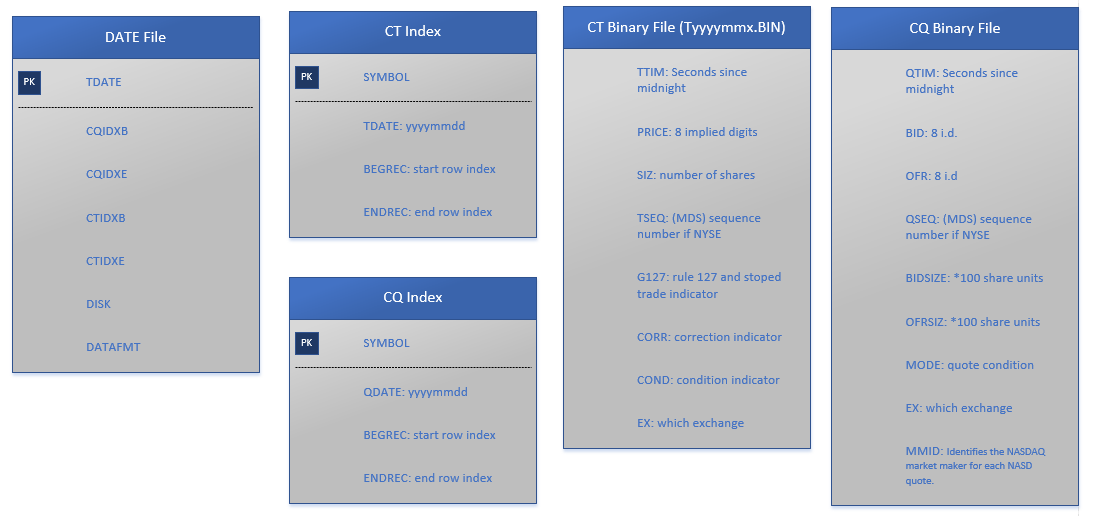
\includegraphics[width=0.7\linewidth]{db1}
\caption[Adatbázis felépítése]{}
\label{fig:db1}
\end{figure}



A projekt alapját képező adathalmaz, mintegy 2.5 terrabájt, egy KDB+ szerveren volt tárolva. Ennek tartalma több évnyi, amerikai tőzsdéken jegyzett vállalatok kereskedési adatai. (T\&Q)
A fájlok egy része ASCII másik rész bináris formátumban volt elérhető. Az évek során a fájlformátum kis mértékben változott.
\subsection{Python}
Az adatbázis lekérdezések automatizálására, és a feladat azon részeire amiket adatbázis-műveletekkel nem lehetett megoldani, egy Python feldolgozó szkriptet hoztam létre. Itt hajtódik végre a Lee-Ready algoritmus, illetve a az adatok exportálása csv formátumban.
\subsection{Wolfram Mathematica}
A modell paramétereinek Maximum Likelihood becslőének kiszámításához a Wolfram Research Mathematica szoftverét használtam. Előnye legfőképpen az volt, hogy szimbolikus algebrával dolgozik, numerikus instabilitás nem jelent problémát.


\section{Eredmények}


\paragraph{IBM}

\begin{center}
	\begin{tabular}{| l | l | l | l |l |}
		\hline
		 & 2004.05.03-09.09 & 2004.09.10-2005.01.18 & 2005.01.19-05.26 & 2005.05.27-10.04 \\ \hline
		$\alpha$ & 0.4202 & 0.4391 & 0.4111 &0.4248 \\ \hline
		$\delta$ & 0.2084 & 0.1206 & 0.5405 &0.2110\\ \hline
		$\epsilon_b$ & 2144 & 2300 & 2478 &2201 \\ \hline
		$\epsilon_b^H$ & 367.9 & 169 & 252.4 &0.0464 \\ \hline
		$\epsilon_s$ & 2413 & 2463 & 2315 &2199 \\ \hline
		$\epsilon_s^H$ & 22.18 & 0.542 & 389.5 &123 \\ \hline
		$\mu$ & 604.1 & 717.5 & 851.626 & 669.6\\ \hline
	\end{tabular}
\end{center}

\paragraph{JNJ}

\begin{center}
	\begin{tabular}{| l | l | l | l |l |}
		\hline
		& 2004.05.03-09.09 & 2004.09.10-2005.01.18 & 2005.01.19-05.26 & 2005.05.27-10.04 \\ \hline
		$\alpha$ 	& 0.0299 	& 0.3223 	& 0.2507&0.4805\\ \hline
		$\delta$ 	& 0.9939	& 0.3604	& 0.1347&0.2376\\ \hline
		$\epsilon_b$ & 2258 	& 2027		& 2136 	&2078 \\ \hline
		$\epsilon_b^H$ & 104.2 	& 253.5		& 112.9 &0.8927 \\ \hline
		$\epsilon_s$ & 1475 	& 1878 		& 2113 &2223 \\ \hline
		$\epsilon_s^H$ & 318.6 	& 112	 	& 1.5489 	&1.892 \\ \hline
		$\mu$ 			&608.7 	& 517.2		& 596.7 & 497.5\\ \hline
	\end{tabular}
\end{center}

\paragraph{PFE}

\begin{center}
	\begin{tabular}{| l | l | l | l |l |}
		\hline
		& 2004.05.03-09.09 & 2004.09.10-2005.01.18 & 2005.01.19-05.26 & 2005.05.27-10.04 \\ \hline
		$\alpha$ 	& 0.4280 	& 0.4053 	& 0.5351 	&0.1110\\ \hline
		$\delta$ 	& 0.5524	& 0.2881 	& 0.8073	&0.9951\\ \hline
		$\epsilon_b$ & 2584		& 2957 		& 3069 		&2472 \\ \hline
		$\epsilon_b^H$ & 107.4	& 466.5 	& 9.796 	&63.54 \\ \hline
		$\epsilon_s$ & 2536 	& 3168 		& 2925  	&2326 \\ \hline
		$\epsilon_s^H$ & 29.82  & 0.1041 	& 0.2837	&191.8 \\ \hline
		$\mu$ 			&479.1  & 717.1		& 734.8 	&641.9\\ \hline
	\end{tabular}
\end{center}

\paragraph{WMT}

\begin{center}
	\begin{tabular}{| l | l | l | l |l |}
		\hline
		& 2004.05.03-09.09 & 2004.09.10-2005.01.18 & 2005.01.19-05.26 & 2005.05.27-10.04 \\ \hline
		$\alpha$ 	& 0.6935 	& 0.4649 	& 0.4705 	&0.3406\\ \hline
		$\delta$ 	& 0.9865	& 0.4602 	& 0.7748 	&0.6359\\ \hline
		$\epsilon_b$ & 2427 	& 2331 		& 2616 		&2430 \\ \hline
		$\epsilon_b^H$ & 283 	& 241.7 	& 148.1 	&35.41 \\ \hline
		$\epsilon_s$ & 1720 	& 2305		& 2575  	&2703 \\ \hline
		$\epsilon_s^H$ & 775 	& 49.03		& 0.2503 	&50.51 \\ \hline
		$\mu$ 			&835.8 	& 559		& 596		& 874.2\\ \hline
	\end{tabular}
\end{center}

\paragraph{XOM}

\begin{center}
	\begin{tabular}{| l | l | l | l |l |}
		\hline
		& 2004.05.03-09.09 & 2004.09.10-2005.01.18 & 2005.01.19-05.26 & 2005.05.27-10.04 \\ \hline
		$\alpha$ 	& 0.4006 	& 0.5800 	& 0.4778	&0.5736\\ \hline
		$\delta$ 	& 0.0376	& 0.7502 	& 0.3487	&0.1032\\ \hline
		$\epsilon_b$ & 2395		& 2514 		& 3277 		&3477 \\ \hline
		$\epsilon_b^H$ & 113.4 	& 271.3 	& 556.4 	&214 \\ \hline
		$\epsilon_s$ & 2422 	& 2369 		& 3148 		&3711 \\ \hline
		$\epsilon_s^H$ & 21.09 	& 1.045		& 365.6 	&3.496 \\ \hline
		$\mu$ 			&697.5 	& 512.6		& 1073	 	& 1026\\ \hline
	\end{tabular}
\end{center}

\section{Forráskód}

https://github.com/kovand11/Msc-Onlab2





\end{document}


